% ********** Software platform **********

\chapter{Software platform}

The software that runs on the Sparrowv3 nodes and the SparrowDongle was
developed by As. Drd. Ing. Andrei Voinescu and is dubbed the SparrowLibrary.
In the process of implementing this protocol we have greatly improved not only
its functionality but its stability and user-friendliness.

The main focus of this library is to provide a C interface for working with the
Sparrow nodes and dongle. It must also be compatible with past and future
Sparrow devices, thus it must support multiple platforms and do this in a
scalable manner. To this end we divided the library into boards and platforms.
Each device must declare exactly one board and one platform, with the board
defining the physical components that make up the device (sensors, LEDs etc.)
and the platform defining the microcontroller (ADC, timers etc.). 

In order to facilitate switching between different devices we used a
cross-platform build system (CMAKE) and divided the library into modules. The
build system allows the user to select the device that his/her code is to be
compiled for and Makefiles will be automatically generated to suit while
modularization of the library means that new code can be easily added to it
while keeping the compilation process fast and the resulting code efficient.

Next we will present some of the most important modules and their
implementation.

\section{Radio module}

This module allows the user to interact with the ATmega128RFA1 radio
transceiver. 

\section{Symbol counter module}

\section{Debug module}

\section{Sleep module}


\begin{figure}[ht]
	\begin{center}
		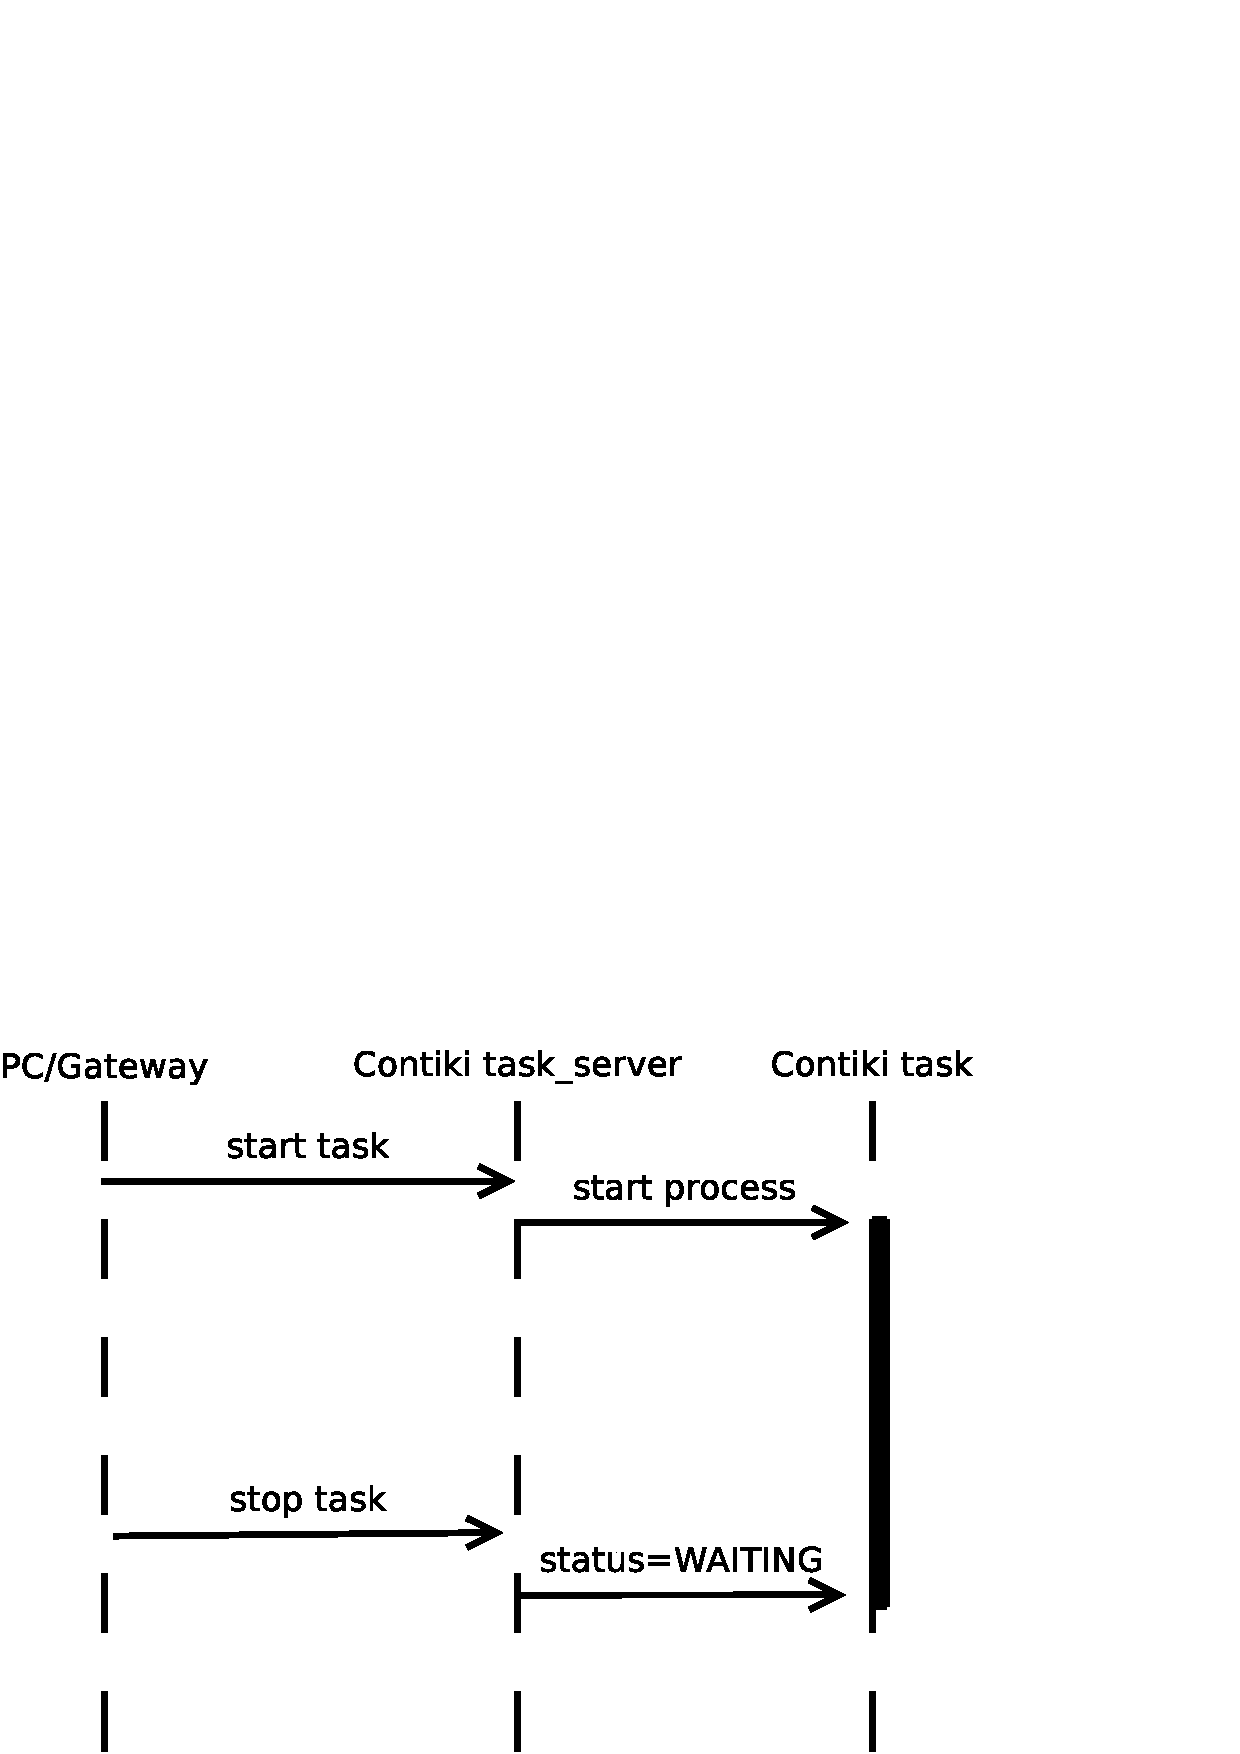
\includegraphics[scale=0.5]{img/starttask.pdf}
	\end{center}
	\caption{\small \itshape{The exchange of messages while starting/stopping tasks}}
\end{figure}

\lstset{numbers=left, mathescape=true, nolol=false,caption=Task server snippet,label=lst:taskserver}
\begin{lstlisting}
PROCESS_THREAD(task_server_process, ev, data)
{
	PROCESS_BEGIN();

	list_init(task_list);

	list_add(task_list,&el_monitor_process);
	list_add(task_list,&el_delay_process);
	list_add(task_list,&el_temperature_sensing);

	tcp_listen(HTONS(1010));

	while(1) 
	{
		PROCESS_WAIT_EVENT_UNTIL(ev == tcpip_event);

		if(uip_connected()) 
		{
			PSOCK_INIT(&ps, buffer, sizeof(buffer));

			while(!(uip_aborted() || uip_closed() 
			|| uip_timedout())) 
			{
				PROCESS_WAIT_EVENT_UNTIL
				(ev == tcpip_event);
				handle_connection(&ps);
			}
		}
	}
	PROCESS_END();
}
\end{lstlisting}

% ********** End of Software platform **********
